%%%%%%%%%%%%%%%%%%%%%%%%%%%%%%%%%%%%%%%%%
% Short Sectioned Assignment
% LaTeX Template
% Version 1.0 (5/5/12)
%
% This template has been downloaded from:
% http://www.LaTeXTemplates.com
%
% Original author:
% Frits Wenneker (http://www.howtotex.com)
%
% License:
% CC BY-NC-SA 3.0 (http://creativecommons.org/licenses/by-nc-sa/3.0/)
%
%%%%%%%%%%%%%%%%%%%%%%%%%%%%%%%%%%%%%%%%%

%----------------------------------------------------------------------------------------
%	PACKAGES AND OTHER DOCUMENT CONFIGURATIONS
%----------------------------------------------------------------------------------------

\documentclass[paper=a4, fontsize=11pt]{scrartcl} % A4 paper and 11pt font size

\usepackage[T1]{fontenc} % Use 8-bit encoding that has 256 glyphs
\usepackage{fourier} % Use the Adobe Utopia font for the document - comment this line to return to the LaTeX default
\usepackage[spanish]{babel} % English language/hyphenation
\usepackage[utf8x]{inputenc}
\usepackage{lipsum} % Used for inserting dummy 'Lorem ipsum' text into the template
\usepackage{graphicx}
\graphicspath{ {images/} }
\usepackage{sectsty} % Allows customizing section commands
\allsectionsfont{\centering \normalfont\scshape} % Make all sections centered, the default font and small caps

\usepackage{fancyhdr} % Custom headers and footers
\pagestyle{fancyplain} % Makes all pages in the document conform to the custom headers and footers
\fancyhead{} % No page header - if you want one, create it in the same way as the footers below
\fancyfoot[L]{} % Empty left footer
\fancyfoot[C]{} % Empty center footer
\fancyfoot[R]{\thepage} % Page numbering for right footer
\renewcommand{\headrulewidth}{0pt} % Remove header underlines
\renewcommand{\footrulewidth}{0pt} % Remove footer underlines
\setlength{\headheight}{13.6pt} % Customize the height of the header


%\setlength\parindent{0pt} % Removes all indentation from paragraphs - comment this line for an assignment with lots of text

%----------------------------------------------------------------------------------------
%	TITLE SECTION
%----------------------------------------------------------------------------------------

\newcommand{\horrule}[1]{\rule{\linewidth}{#1}} % Create horizontal rule command with 1 argument of height

\title{	
\normalfont \normalsize 
\textsc{Universidad de Castilla La Mancha. Sistemas de Información Empresariales.} \\ [25pt] % Your university, school and/or department name(s)
\horrule{0.5pt} \\[0.4cm] % Thin top horizontal rule
\huge Artículo 3. Using OLAP and multidimensional data for decision making \\ % The assignment title
\horrule{2pt} \\[0.5cm] % Thick bottom horizontal rule
}

\author{José María García García} % Your name

\date{\normalsize\today} % Today's date or a custom date

\begin{document}

\maketitle % Print the title

%----------------------------------------------------------------------------------------
%	PROBLEM 1
%----------------------------------------------------------------------------------------

\section{Preguntas}

Leer el artículo y obtener de él información acerca de los siguientes puntos.

\begin{itemize}
\item \textbf{ ¿Qué dos sistemas puede utilizar un gestor para obtener un mejor conocimiento de su empresa?}
\end{itemize}
Procesamiento Analítico En Línea (On-Line Analytical Processing, OLAP) y Bases de Datos de Múltiples Dimensiones (MultiDimensional DataBases, MDDB). Las bases se utilizan para guardar datos que se usarán en análisis (ya veremos porque estas bases son mejor que las relacionales para esta finalidad) y con los sistemas OLAP manipulamos la información de dichas bases. Los sistemas OLAP nos presentan la información resumida que han extraído de bases de múltiples dimensiones y nos permiten estudiar los datos que contienen, trocear los datos para estudiar un aspecto de los mismos, etc. 

\begin{itemize}
\item \textbf{¿Qué diferencia hay entre los sistemas OLTP y OLAP?}
\end{itemize}
Los sistemas OLTP son Sistemas de Procesamiento de Transacciones En Línea (On-Line Transaction Processing), por lo que están centrados en las operaciones del día a día de la empresa, y no tanto en el análisis de los datos que generan esas transacciones. Aunque estos sistemas suelen incorporar mecanismos para generar informes según las actividades de la empresa, estos no sirven para tener una visión general ni para apreciar rápidamente puntos fuertes y puntos débiles. Además, son informes cuya lectura resulta tediosa y los gestores no suelen leerlos. 

\begin{itemize}
\item \textbf{A la hora de obtener información sobre el funcionamiento general de la empresa, ¿qué características tiene el tipo de sistema preferido por los gestores?}
\end{itemize}
A diferencia del sistema comentado anteriormente, un sistema que usa OLAP y MDDB es intuitivo, fácil de usar y está orientado a la búsqueda de información de tal forma que permita, mediante un vistazo rápido, saber que está pasando en la empresa y formarse una idea general sobre la misma.
%%%
%%%%%%%%%%%%%%%% OJO A JUGAR PARA LAS COMILLAS DOBLES
%%%

\begin{itemize}
\item \textbf{¿Cómo se representa la información cuando utilizamos una base de datos multidimensional?. Indica un ejemplo}
\end{itemize}
La información se representa mediante arrays (vectores, listas) de varias dimensiones. A la estructura que toman los datos en la base se la llama \textbf{hipercubo}, aunque esta puede no tener forma de cubo, esto es, si el array en cuestión tiene una dimensión 4, no podemos representar esa estructura como un tetraedro, ya que para ello el array debería ser de dimensión 3. Estas estructuras son preferidas a otras porque permiten ``jugar'' con la información para observarla desde muchos puntos de vista diferentes, centrar el análisis en un único aspecto de los datos, etc. El uso más simple de estas bases es el que podemos observar en el ejemplo.
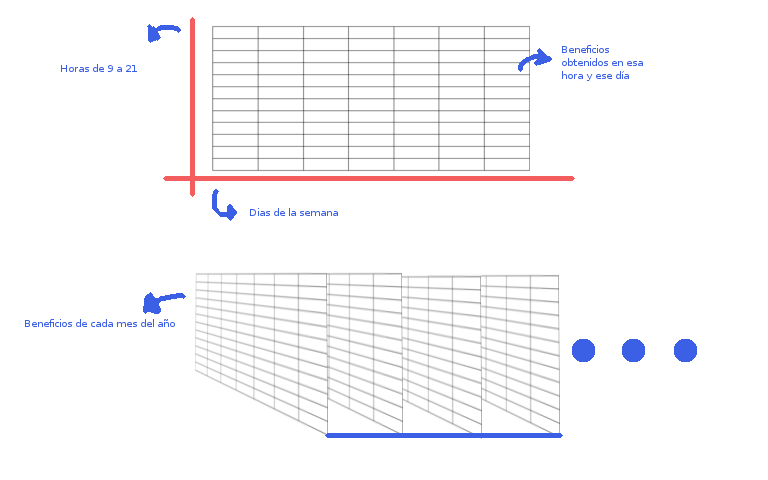
\includegraphics[scale=0.75]{ejemplo}
\newline
En este caso, el dato a estudiar ha sido el beneficio que obtiene la empresa y las variables según las cuales lo hemos estudiado han sido la hora del día, el día de la semana y el mes del año. Esta representación permite ver como varían los datos según cada una de las variables, localizar los puntos donde se detecten perdidas y arreglarlos, etc. Cabe también destacar que cada valor de beneficio está identificado de forma unívoca por sus coordenadas en el cubo (mes, día, hora).

\begin{itemize}
\item \textbf{¿Por qué las base de datos relacionales son adecuadas para almacenar información transaccional y no analítica?}
\end{itemize}
Porque estas bases permiten guardar información de las transacciones de forma rápida y sencilla, información que luego se puede estudiar con los informes autogenerados o a través de órdenes SQL. No obstante, dada la fragmentación y volumen que presentan los datos usados en analítica, manejar estas bases de datos dejaba de ser una trivialidad, por lo que para analítica se prefieren las MDDB.

\begin{itemize}
\item \textbf{¿Qué tipo de información suele almacenarse en las base de datos multidimensionales?}
\end{itemize}
Los datos comúnmente almacenados en estas bases de datos suelen ser numéricos y muestran el rendimiento que ha tenido la empresa u organización a lo largo de su historia. Estos datos provienen de otras bases de la empresa, que se vuelcan en la base multidimensional y esta limpia, resume y procesa la información para el uso de los gestores.

\begin{itemize}
\item \textbf{ ¿Qué tipo de interactividad es permitida sobre los datos de una base de datos multidimensional?¿Qué tipo de aplicaciones permiten esta interactividad?}
\end{itemize}
Siguiendo la metáfora del cubo respecto a la representación de la información, el cubo puede \textbf{hacerse rodajas}, para observar los valores de los datos respecto a un valor concreto de una de las coordenadas de los mismos. Estas rodajas pueden \textbf{trocearse} además para observar la información enmarcada en un rango de valores. Podemos observar cuadrados concretos del cubo o subconjuntos del mismo. Podemos pasar el cubo por un \textbf{filtro} para quedarnos con los bloques que satisfagan ese filtro. Normalmente esto se hace mediante interfaces gráficas, lo que hace el análisis más ameno que la lectura de un informe. Al conjunto de herramientas que se usan para esa manipulación del cubo se les llama OLAP. 

\begin{itemize}
\item \textbf{¿Qué opciones tenemos a la hora de implantar una MDDB? ¿En qué se centra cada una de ellas?}
\end{itemize}
Existen dos enfoques a la hora de implementar una MDDB:
\begin{enumerate}
\item \underline{Enfoque top-down (de arriba a abajo)}: centrado en la planificación del negocio.
\item \underline{Enfoque bottom-up (de abajo a arriba)}: centrado en bases y sistemas existentes.
\end{enumerate}

\begin{itemize}
\item \textbf{ ¿En qué consiste el ``síndrome de los datos disponibles''?}
\end{itemize}
Es un síndrome en el que se puede caer al usar como enfoque de implementación el bottom-up, que implica que al partir de datos y sistemas que ya existen, se intenta crear una base que lo contenga todo y lo tenga disponible para todos, cuando realmente eso no es necesario.

\begin{itemize}
\item \textbf{ ¿Qué pasos se dan en una implantación top-down?}
\end{itemize}
En este proceso de implementación se empieza desde arriba, es decir, partimos de lo que la empresa quiere y para qué lo quiere. 
	\begin{itemize}
		\item Se lleva a cabo una \textbf{elicitación de requisitos}, proveidos por el gestor de la empresa o negocio. 
		\item El desarrollador determina las \textbf{medidas} de la MDDB en base a esos requisitos.
		\item Se prepara un \textbf{prototipo} de MDDB que se muestra a la empresa haciendo uso de un software OLAP. 
	\end{itemize}
Este enfoque asegura que la base que se desarrolle se ajustará a las necesidades de la empresa, lo que no siempre es bueno, ya que la base se desarrollará exclusivamente para un fin concreto, además de que se hará sin tener en cuenta los sistemas sobre los que se apoya, lo que puede dar lugar a problemas si no se prevén posibles modificaciones que puedan sufrir las bases subyacentes durante el desarrollo de la MDDB. 

\begin{itemize}
\item \textbf{¿Qué pasos se dan en una implantación bottom-up?}
\end{itemize}
En este tipo de implementación partimos de unos datos que ya existen en unas bases de datos de una tecnología concreta, es decir, empezamos la implementación por abajo. En este enfoque, aunque nos guiamos por requisitos también, empezamos la implementación fijándonos en el origen de los datos, de manera que estos determinarán como será la MDDB. Los pasos que se dan en este enfoque son los siguientes:
\begin{itemize}
	\item El primer paso es \textbf{analizar dichos datos y tomar medidas} para la confección de la base de datos multidimensional. Esta toma de medidas da lugar a lo que se conoce como diagrama en estrella, que contiene dos tipos de tablas:
	\begin{itemize}
	\item \textbf{Tabla de hecho}, formada por datos numéricos que existen dentro de la base de datos.
	\item \textbf{Tablas de dimensiones}, formadas por datos más descriptivos que se pueden asociar a las dimensiones de la base dentro de la empresa.
	\end{itemize}
	\item Haciendo uso de este diagrama, se \textbf{traduce} la base de datos relacional a una MDDB, ya que permite concretar el tema central del análisis. Esta traducción es también una simplificación y puede incluso automatizarse. 
\end{itemize}	
El problema que tiene este enfoque es que hacer esa traducción es una tarea de lo más complicada, incluso para expertos cualificados (además durante la ejecución de esta actividad se puede caer en el síndrome mencionado anteriormente). 

\begin{itemize}
\item \textbf{¿Qué enfoque alternativo puede plantearse? ¿En qué consiste?}
\end{itemize}
Existe un enfoque alternativo a estos dos que es realmente una media de ambos. Dado que podríamos considerar el enfoque top-down como un enfoque centrado en el usuario y el bottom-up como un enfoque centrado en el desarrollador, podríamos considerar este enfoque como uno orientado a ambas figuras y que consta de los siguientes pasos.
	\begin{enumerate}
	\item Elegir un gestor apto para ejercer el rol de representante del proyecto (en el lado de la empresa). Extraer de este representante las necesidades de la empresa.
	\item Localizar las fuentes de datos necesarias para tomar las medidas de la MDDB e identificar un subconjunto de los datos a modo de muestra con el que se pueda trabajar fácilmente.
	\item Identificar los datos que el representante no haya identificado inicialmente y comentarlos con él (quizá suponga una ventaja incluir esos datos en la base y el representante simplemente olvidó comentarlo).
	\item Desechar datos que no sean esenciales, para evitar sufrir el síndrome de los datos disponibles.
	\item Construir un prototipo de la MDDB y que lo revisen tanto el representante del proyecto como los gestores de las bases de datos actuales.
	\item Si el gestor mencionado lo considera, modificar las fuentes de datos para facilitar la extracción a la MDDB.
	\end{enumerate}
Este enfoque tiene partes tanto top-down, en las que se determina que información nos interesa controlar y analizar, como bottom-up, en fases en las cuales los datos y sus fuentes determinan los datos que estarán disponibles así como la forma en la que se modelará la información. A pesar de ser un enfoque intermedio, no es tampoco la opción perfecta en todas las situaciones.

\end{document}